\section{Risposte alle domande}

\subsection{Domanda 1}
\textit{Misurate i tempi di calcolo dell'algoritmo deterministico di Stoer e Wagner sui grafi del dataset. Mostrate i risultati con un grafico che mostri la variazione dei tempi di calcolo al variare del numero di vertici nel grafo. Confrontate i tempi misurati con la complessità asintotica dell'algoritmo. \\
Nelle istanze più grandi, il tempo di calcolo necessario per completare l'esecuzione potrebbe risultare eccessivo. In questo caso utilizzate un timeout, riportando nei risultati che l'algoritmo non riesce ad ottenere un risultato in tempo utile.}

Abbiamo implementato il codice in Python per l'esecuzione dell'algoritmo di Stoer-Wagner su tutto il dataset fornito. I risultati, che sono stati riportati in modo dettagliato con i relativi pesi anche nella sezione appendice, sono riportati di seguito.

\begin{figure}[H]
	\centering
	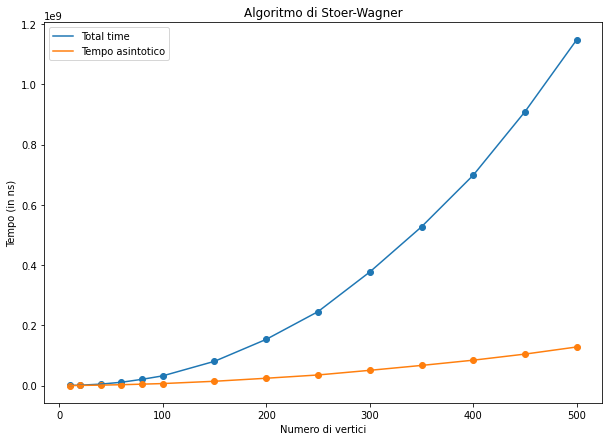
\includegraphics[width=0.85\textwidth]{res/images/single/stoerwagner}
	\caption{Complessità di Stoer-Wagner con \textit{k} esecuzioni ripetute per ogni quartetto di grafi con uguale numero di nodi.}
	\label{fig:stoerwagner}
\end{figure}

Nel grafico appena illustrato (fig. \ref{fig:stoerwagner}) è riportata la complessità computazionale attesa (in giallo) ed effettiva (in blu) per l'algoritmo di Stoer e Wagner con più esecuzioni dell'algoritmo. \\
Come si può evincere dall'immagine, la complessità dell'algoritmo da noi implementato ricalca quasi alla perfezione quella teorica. Questo è probabilmente dovuto alle ottimizzazioni che sono state implementate, prime tra tutte l'ottimizzazione della copia profonda e l'utilizzo della mappa degli indici in \texttt{MaxHeap}. Per questo motivo, non è stato necessario impostare un timeout per bloccare l'esecuzione dell'algoritmo. % weird flex but ok

\subsection{Domanda 2}
\textit{Misurate i tempi di calcolo dell'algoritmo di Karger e Stein sui grafi del dataset, usando un numero di ripetizioni che garantisca una probabilità minore o uguale a $1/n$ di sbagliare. Mostrate i risultati con un grafico che mostri la variazione dei tempi di calcolo al variare del numero di vertici nel grafo. Confrontate i tempi misurati con la complessità asintotica dell'algoritmo. \\
Nelle istanze più grandi, il tempo di calcolo necessario a completare tutte le iterazioni potrebbe risultare eccessivo. In questo caso utilizzate un timeout oppure abbassate il numero di ripetizioni per ottenere tempi di esecuzione ragionevoli.}

\subsubsection{Analisi della complessità}

Analogamente a Stoer-Wagner, anche per Karger-Stein abbiamo 
implementato il codice in Python per l'esecuzione dell'algoritmo su tutto il dataset 
fornito. I risultati, che sono stati riportati in modo dettagliato con i relativi pesi 
anche nella sezione appendice, sono riportati di seguito.
Nel grafico \ref{fig:kargerstein} è riportata la complessità 
computazionale teorica (in giallo) ed effettiva (in blu) per l'algoritmo di Karger e 
Stein, con più esecuzioni dell'algoritmo. È possibile notare dall'immagine che la 
complessità dell'algoritmo da noi implementato rimane al di sotto della complessità 
teorica, pur mantenendo un andamento molto simile. In particolare, il tempo richiesto 
per l'esecuzione dell'ultima istanza risulta essere molto simile al tempo previsto 
dalla complessità teorica.

Oltre alle ripetizioni necessarie per effettuare le misurazioni correttamente 
(si veda \S\ref{guida_misurazioni}), l'algoritmo di Karger-Stein richiede che il 
procedimento descritto precedentemente (si veda \S\ref{karger_stein_section}) venga 
ripetuto un numero sufficiente di volte, tale per cui l'algoritmo ha una probabilità 
minore o uguale a $\frac{1}{n}$ di sbagliare. Pertanto, il numero di ripetizioni che 
soddisfa questo vincolo è pari a $log^{2}(n)$.

\begin{figure}[H]
	\centering
	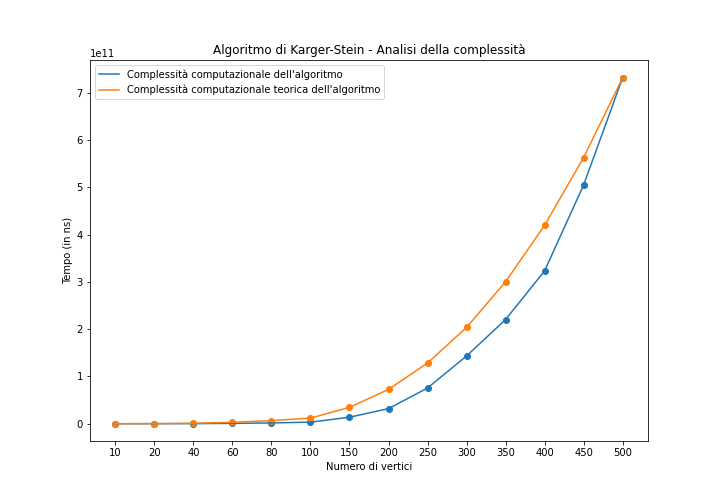
\includegraphics[width=1\textwidth]{res/images/single/karger-stein/complexity/karger_stein_complexity.png}
	\caption{Complessità di Karger-Stein con \textit{k} esecuzioni ripetute per ogni quartetto di grafi con uguale numero di nodi.}
	\label{fig:kargerstein}
\end{figure}

\subsubsection{Introduzione di una soglia sul tempo di esecuzione dell'algoritmo}

È possibile notare che questo algoritmo impiega molto tempo per computare le istanze 
che hanno un numero di vertici superiore a 250. Per questo motivo è stato 
deciso di svolgere un'analisi riguardo la scelta di uno o più appositi valori come 
soglia sul tempo di esecuzione dell'algoritmo. Per determinare tali valori sono stati 
osservati i vari discovery time per le varie istanze. È stato possibile notare che 
svolgendo una \textit{media aritmetica} dei discovery time l'algoritmo 
impiega 4.5 secondi per determinare il min-cut (circa il 7.56\% del tempo totale 
di esecuzione dell'algoritmo). Tuttavia, scegliere come \textit{threshold} questo 
valore, poteva andare a penalizzare la qualità delle soluzioni per quanto riguarda 
i grafi con un numero di vertici maggiore di 250. Quindi, si è proceduti nel calcolare 
anche la \textit{media ponderata} dei discovery time, ottenendo un valore pari a 
circa 9 secondi. A seguito di questa analisi, sono state svolte due misurazioni: una 
misurazione con una soglia impostata a 6 secondi sul tempo di esecuzione totale 
dell'algoritmo e una con una soglia di 10 secondi. Sono stati scelti dei valori 
leggermente maggiori rispetto ai valori forniti dalle medie in quanto potevano 
essere troppo stringenti per le istanze più grandi.

\begin{figure}[H]
	\centering
	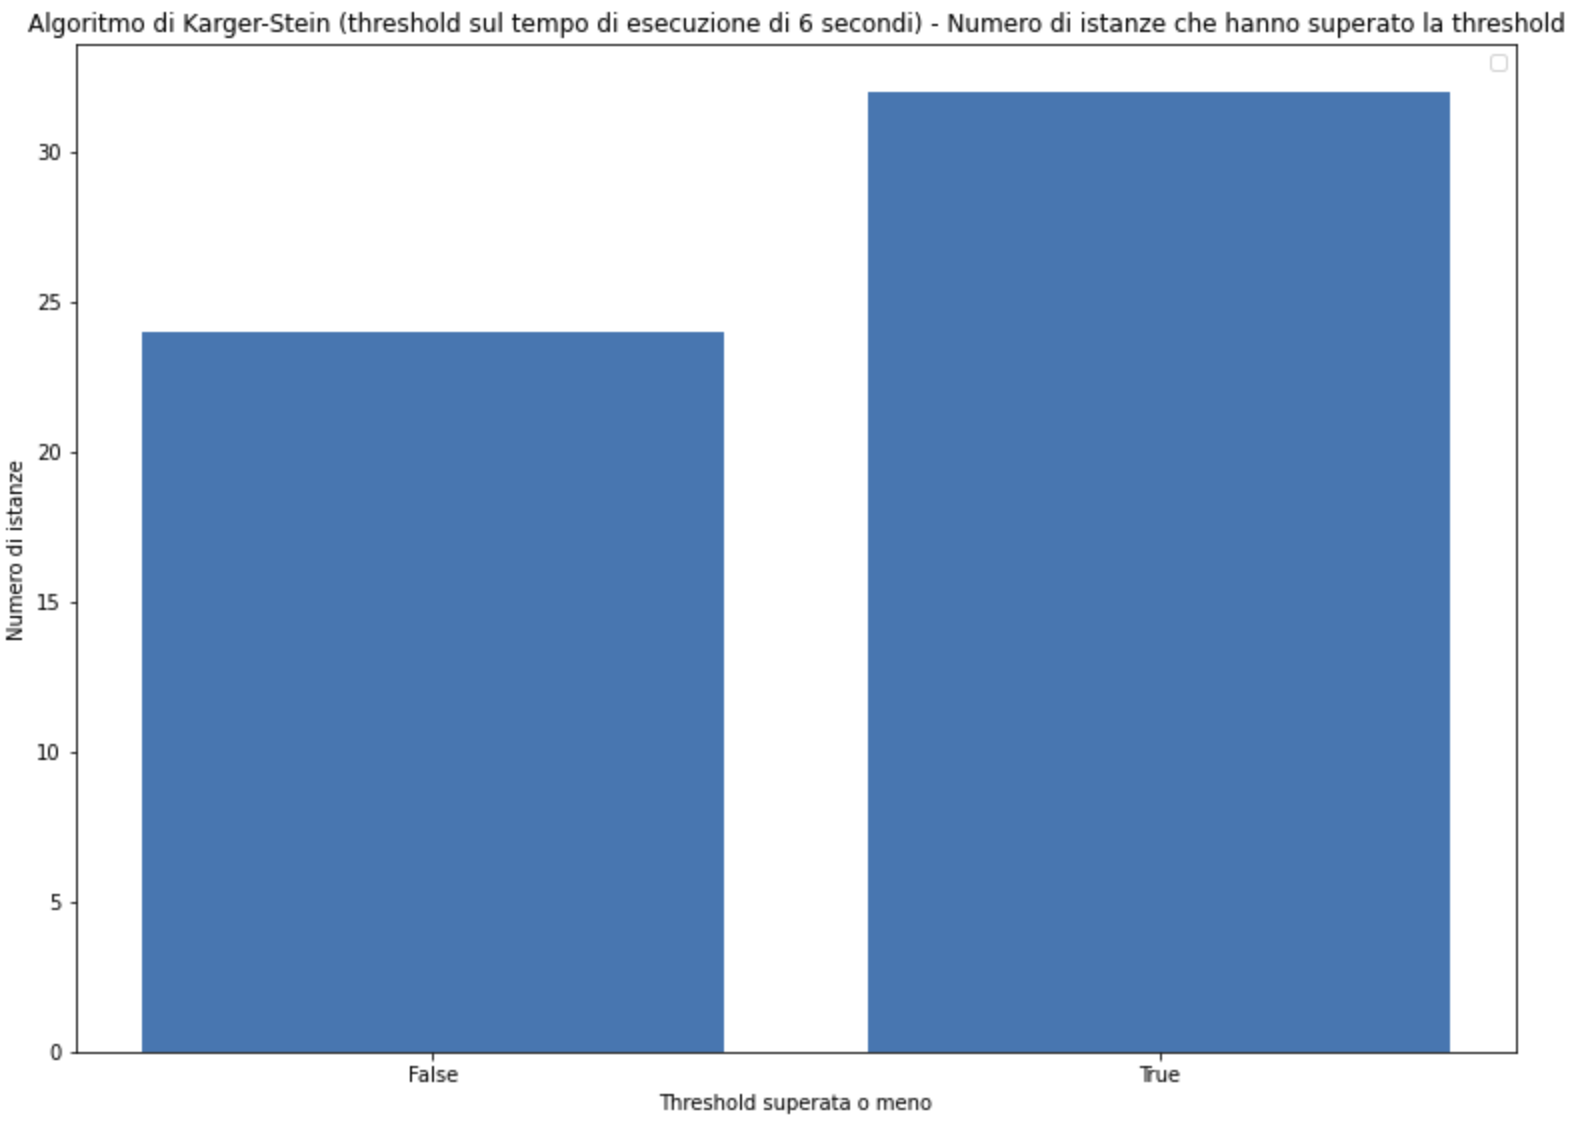
\includegraphics[width=0.6\textwidth]{res/images/single/karger-stein/karger_stein_istanze_superato_threshold_6s.png}
	\caption{Numero di istanze che hanno superato la soglia di 6 secondi.}
	\label{fig:karger_stein_istanze_superato_threshold_6s}
\end{figure}

\begin{figure}[H]
	\centering
	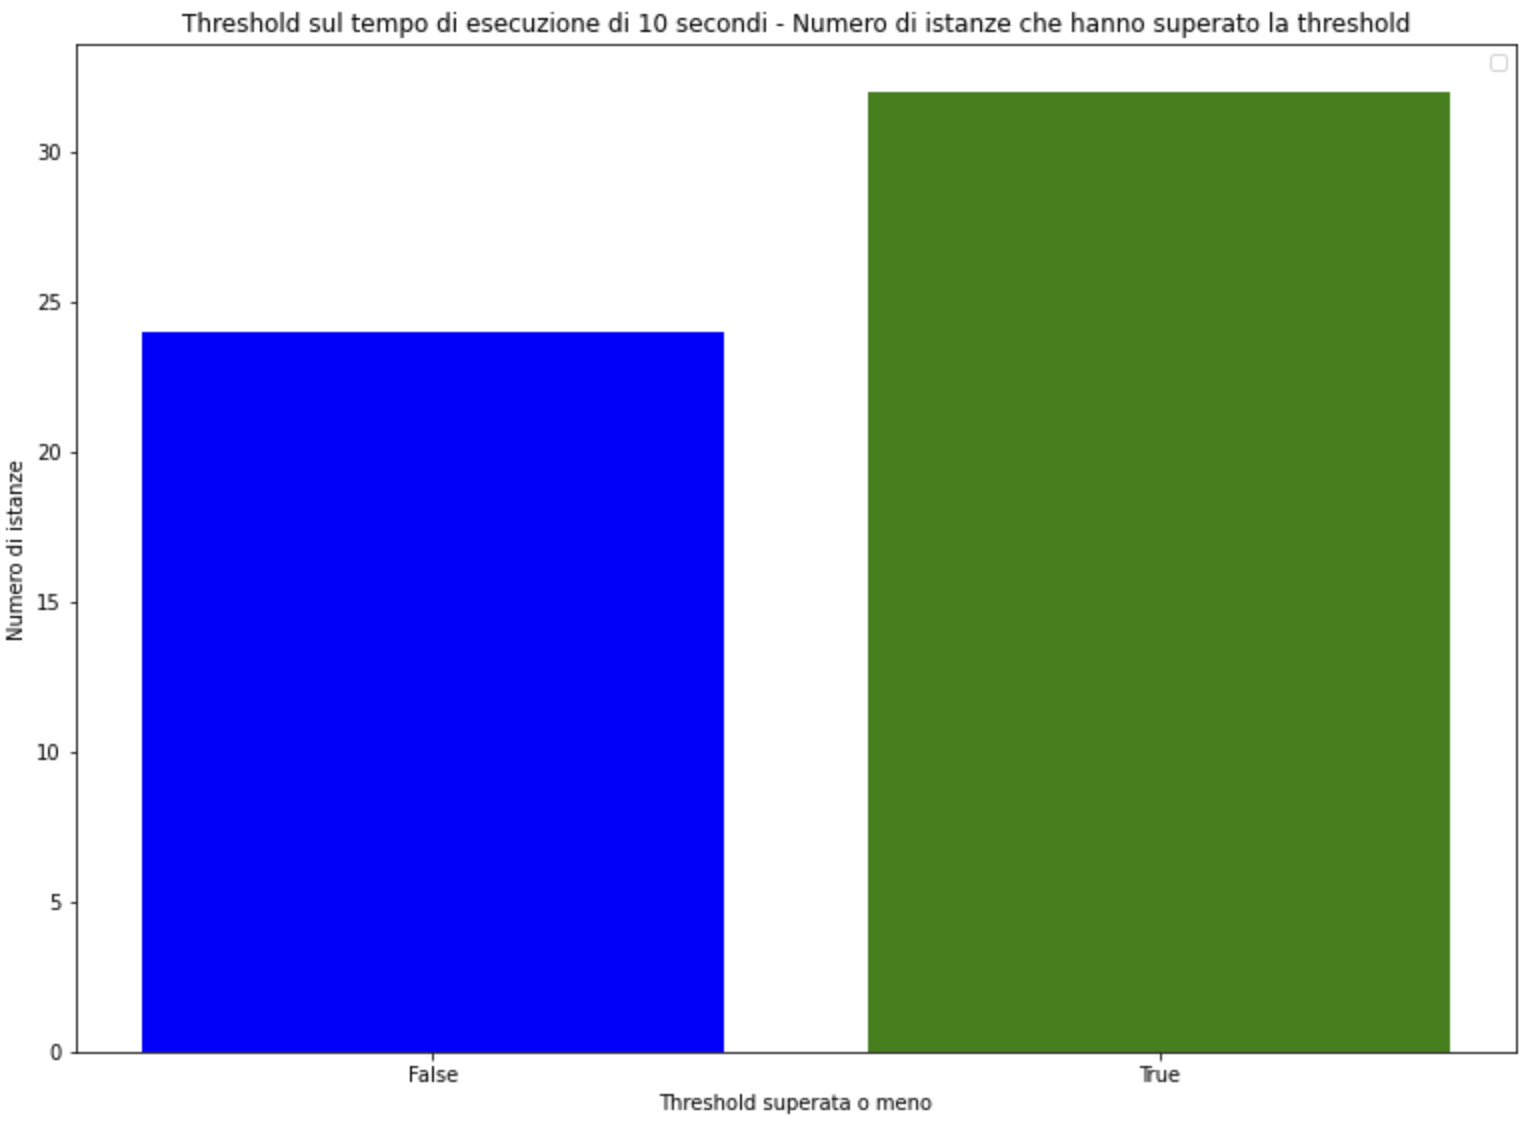
\includegraphics[width=0.6\textwidth]{res/images/single/karger-stein/karger_stein_istanze_superato_threshold_10s.png}
	\caption{Numero di istanze che hanno superato la soglia di 10 secondi.}
	\label{fig:karger_stein_istanze_superato_threshold_10s}
\end{figure}

Nelle risposte alle successive domande, pertanto, sarà possibile vedere il confronto 
tra tre possibili esecuzioni dell'algoritmo: un'esecuzione senza alcuna soglia sul 
tempo, un'esecuzione con una soglia di 6 secondi e un'esecuzione con una soglia di 10 
secondi.

\subsubsection{Altre analisi}

Un'altra analisi che è stata effettuata, ma che non abbiamo utilizzato per fare ulteriori misurazioni, riguarda il numero di iterazioni minime in cui l'algoritmo  
riesce a determinare il min-cut. È stato possibile notare che rispetto alle $log^{2}(n)$ 
ripetizioni che l'algoritmo necessita per l'\textit{alta probabilità}, l'algoritmo 
era in grado di determinare il min-cut in un numero di iterazioni molto minore rispetto a 
$log^{2}(n)$. Analogamente per quanto riguarda i discovery time, facendo la media 
aritmetica del numero di iterazioni minime si è ottenuto un valore pari a 2.6 
(circa il 7.39\% delle ripetizioni totali), mentre facendo la media ponderata si è 
ottenuto un valore pari a 2.2. La differenza non è sostanziale, pertanto è stato 
deciso di focalizzare l'attenzione nell'analisi dell'algoritmo introducendo delle 
soglie sul tempo di esecuzione. Si illustrino dei grafici inerenti all'analisi appena 
descritta:

\begin{figure}[H]
	\begin{subfigure}{.5\textwidth}
		\centering
		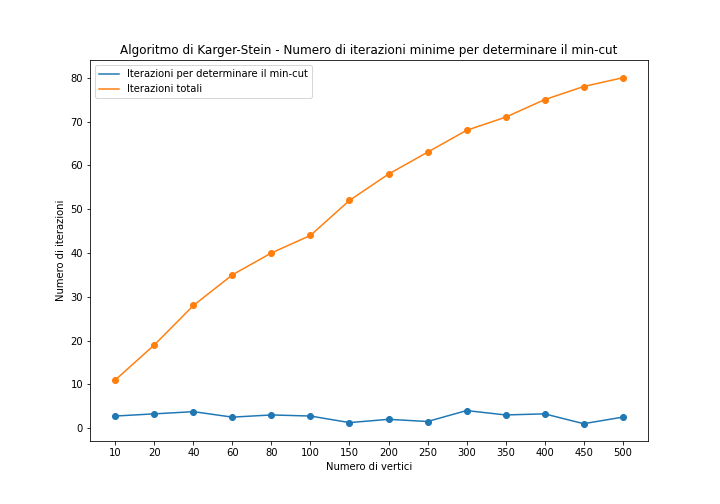
\includegraphics[width=1\textwidth]{res/images/single/karger-stein/iterazioni/karger_stein_confronto_numero_iterazioni.png}
		\caption{Confronto tra il numero di iterazioni minime in cui l'algoritmo è 
		riuscito a determinare il min-cut e il numero di iterazioni totali.}
		\label{fig:karger_stein_confronto_numero_iterazioni}
	\end{subfigure}
	\begin{subfigure}{.5\textwidth}
		\centering
		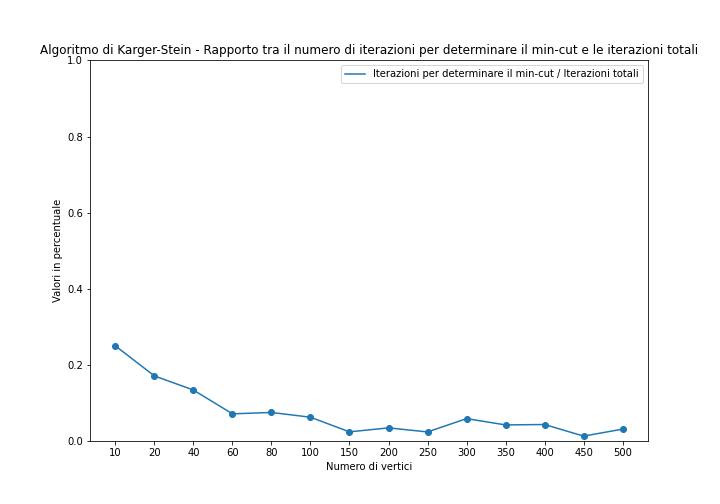
\includegraphics[width=1\textwidth]{res/images/single/karger-stein/iterazioni/karger_stein_rapporto_numero_iterazioni.png}
		\caption{Rapporto tra il numero di iterazioni minime in cui l'algoritmo è 
		riuscito a determinare il min-cut e il numero di iterazioni totali.}
		\label{fig:karger_stein_rapporto_numero_iterazioni}
	\end{subfigure}
	\caption{Analisi del numero di iterazioni minime in cui l'algoritmo riesce a 
	determinare il min-cut.}
	\label{fig:karger_stein_numero_iterazioni}
\end{figure}

\subsection{Domanda 3}
\textit{Misurate il discovery time dell'algoritmo di Karger e Stein sui grafi del dataset. Il discovery time è il momento (in secondi) in cui l'algoritmo trova per la prima volta il taglio di costo minimo.  Confrontate il discovery time con il tempo di esecuzione complessivo per ognuno dei grafi nel dataset.}

\begin{figure}[H]
	\begin{subfigure}{.49\textwidth}
		\centering
		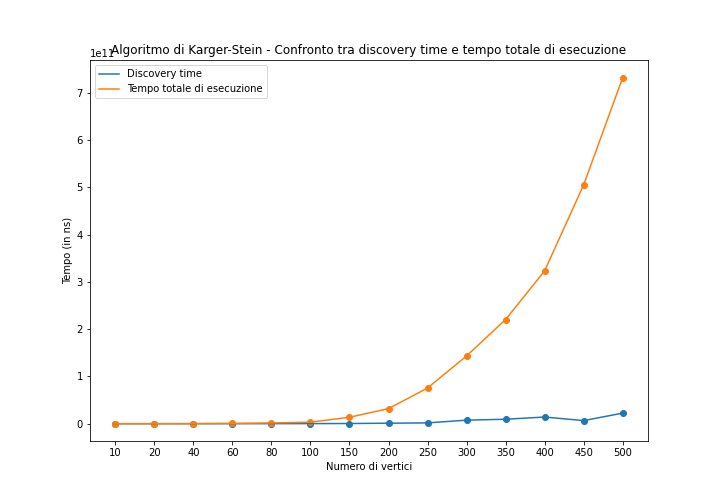
\includegraphics[width=1\textwidth]{res/images/single/karger-stein/discovery-time/karger_stein_confronto_discovery_time_total_time.png}
		\caption{Confronto tra il tempo totale di esecuzione dell'algoritmo e il discovery time per ogni esecuzione.}
		\label{fig:karger_stein_confronto_discovery_time_total_time}
	\end{subfigure}
	\begin{subfigure}{.49\textwidth}
		\centering
		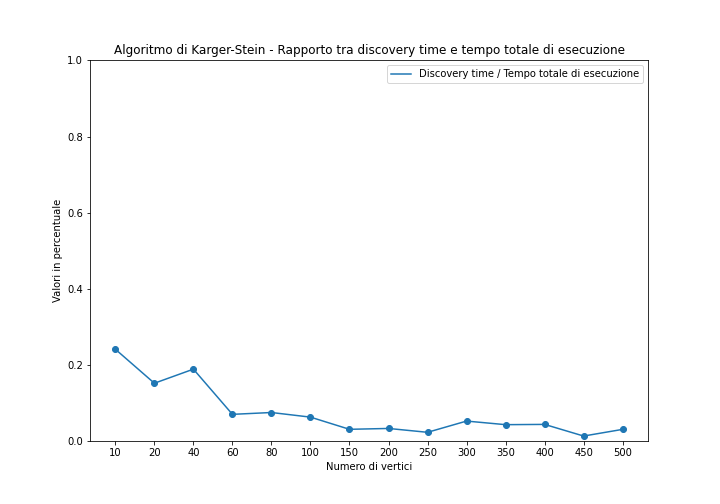
\includegraphics[width=1\textwidth]{res/images/single/karger-stein/discovery-time/karger_stein_rapporto_discovery_time_total_time.png}
		\caption{Rapporto tra il tempo totale di esecuzione dell'algoritmo 
		e il discovery time per ogni esecuzione.}
		\label{fig:karger_stein_rapporto_discovery_time_total_time}
	\end{subfigure}
	\caption{Esecuzione dell'algoritmo di Karger-Stein senza una threshold sul tempo.}
	\label{fig:karger_stein_discovery_time}
\end{figure}

I valori del grafico \ref{fig:karger_stein_rapporto_discovery_time_total_time} 
esprimono la percentuale di tempo impiegato per trovare per la prima 
volta il min-cut, rispetto al tempo totale di esecuzione dell'algoritmo.
Dai grafici è possibile notare che per le istanze più piccole, il rapporto 
tra il discovery time e il tempo totale di esecuzione è maggiore rispetto 
allo stesso rapporto per le istanze più grandi.
L'esecuzione dell'algoritmo con la threshold a 10 secondi (grafici 
\ref{fig:karger_stein_discovery_time_threshold_10s}) impiega, in media, un tempo maggiore per determinare il min-cut. È possibile notare che 
l'esecuzione dell'algoritmo senza threshold impiega un tempo maggiore rispetto 
alle esecuzioni con la threshold. Questo perché le istanze più grandi richiedono 
un tempo maggiore per poter determinare il min-cut. Tuttavia, l'esecuzione senza 
threshold non ha prodotto errori rispetto al min-cut ottimo. Il tempo medio del 
discovery time è:
\begin{enumerate}
	\item \textit{Senza threshold}: 4.5 secondi (7.56\% del tempo totale di 
	esecuzione dell'algoritmo);
	\item \textit{Threshold di 6 secondi}: 2.7 secondi (38.42\% del tempo totale di 
	esecuzione dell'algoritmo);
	\item \textit{Threshold di 10 secondi}: 3.1 secondi (29.87\% del tempo totale di 
	esecuzione dell'algoritmo).
\end{enumerate}

\pagebreak

\noindent Di seguito si illustrano i grafici inerenti ai discovery time con le diverse soglie 
(grafici \ref{fig:karger_stein_discovery_time_threshold_6s}, 
\ref{fig:karger_stein_discovery_time_threshold_10s}, 
\ref{fig:karger_stein_discovery_time_thresholds}):

\begin{figure}[H]
	\begin{subfigure}{.5\textwidth}
	  \centering
	  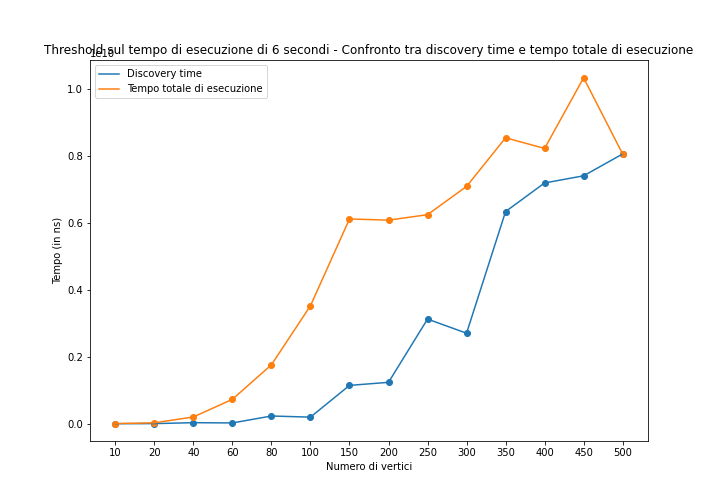
\includegraphics[width=1\textwidth]{res/images/single/karger-stein/discovery-time/threshold6/karger_stein_confronto_discovery_time_total_time_threshold_6s.png}
	  \caption{Confronto tra il tempo totale di esecuzione dell'algoritmo e il discovery time per ogni esecuzione.}
	  \label{fig:karger_stein_confronto_discovery_time_total_time_threshold_6s}
	\end{subfigure}
	\begin{subfigure}{.5\textwidth}
	  \centering
	  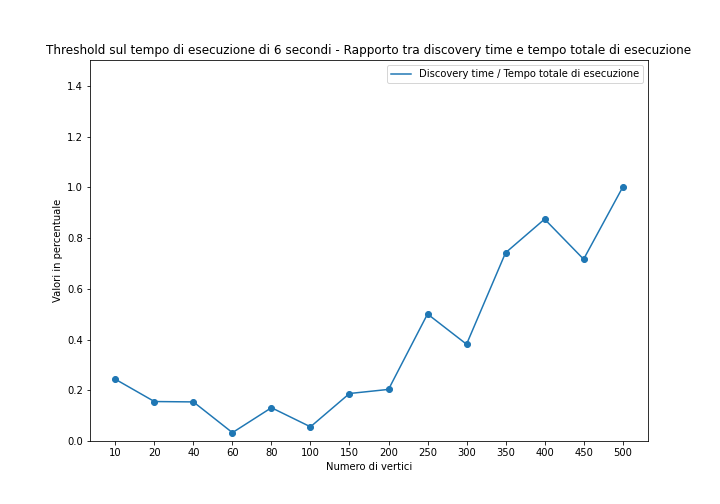
\includegraphics[width=1\textwidth]{res/images/single/karger-stein/discovery-time/threshold6/karger_stein_rapporto_discovery_time_total_time_threshold_6s.png}
	  \caption{Rapporto tra il tempo totale di esecuzione dell'algoritmo 
	  e il discovery time per ogni esecuzione.}
	  \label{fig:karger_stein_rapporto_discovery_time_total_time_threshold_6s}
	\end{subfigure}
	\caption{Esecuzione dell'algoritmo di Karger-Stein con una threshold sul tempo di 
	6 secondi.}
	\label{fig:karger_stein_discovery_time_threshold_6s}
\end{figure}

\begin{figure}[H]
	\begin{subfigure}{.5\textwidth}
	  \centering
	  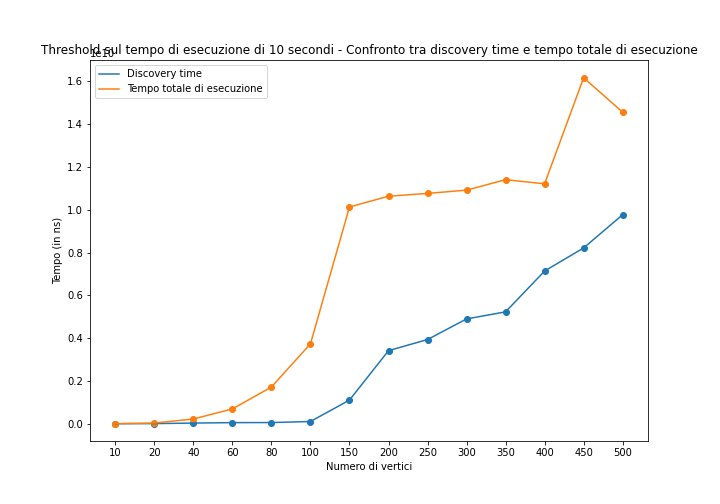
\includegraphics[width=1\textwidth]{res/images/single/karger-stein/discovery-time/threshold10/karger_stein_confronto_discovery_time_total_time_threshold_10s.png}
	  \caption{Confronto tra il tempo totale di esecuzione dell'algoritmo e il discovery time per ogni esecuzione.}
	  \label{fig:karger_stein_confronto_discovery_time_total_time_threshold_10s}
	\end{subfigure}
	\begin{subfigure}{.5\textwidth}
	  \centering
	  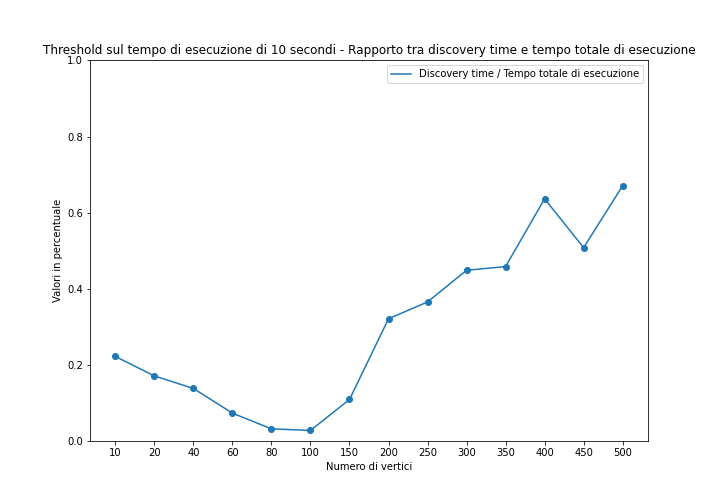
\includegraphics[width=1\textwidth]{res/images/single/karger-stein/discovery-time/threshold10/karger_stein_rapporto_discovery_time_total_time_threshold_10s.png}
	  \caption{Rapporto tra il tempo totale di esecuzione dell'algoritmo e il 
	  discovery time per ogni esecuzione.}
	  \label{fig:karger_stein_rapporto_discovery_time_total_time_threshold_10s}
	\end{subfigure}
	\caption{Esecuzione dell'algoritmo di Karger-Stein con una threshold sul tempo di 
	10 secondi.}
	\label{fig:karger_stein_discovery_time_threshold_10s}
\end{figure}

\begin{figure}[H]
	\begin{subfigure}{.5\textwidth}
	  \centering
	  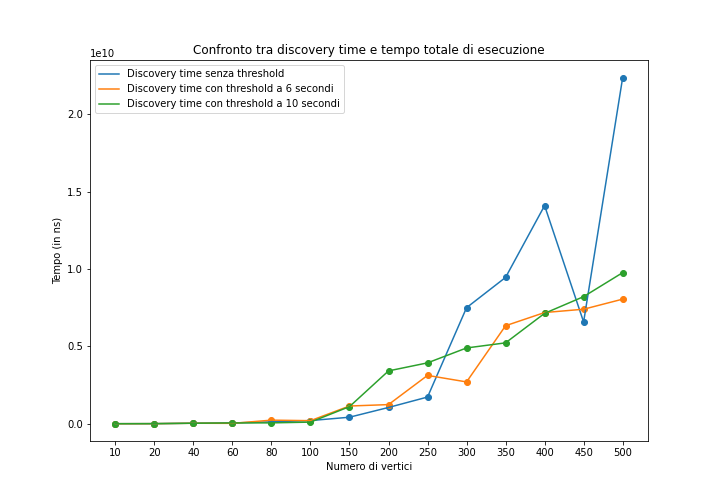
\includegraphics[width=1\textwidth]{res/images/single/karger-stein/discovery-time/confronto/karger_stein_confronto_discovery_time_total_time_with_thresholds.png}
	  \caption{Confronto tra il tempo totale di esecuzione dell'algoritmo e il discovery time per ogni esecuzione.}
	  \label{fig:confronto}
	\end{subfigure}
	\begin{subfigure}{.5\textwidth}
	  \centering
	  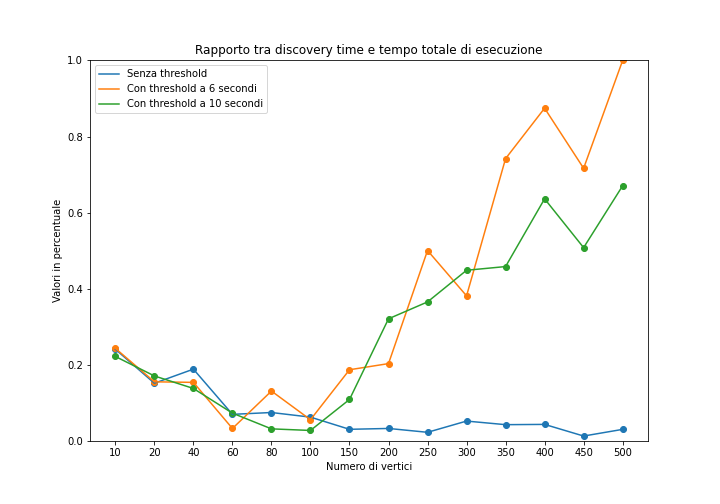
\includegraphics[width=1\textwidth]{res/images/single/karger-stein/discovery-time/confronto/karger_stein_rapporto_discovery_time_total_time_with_thresholds.png}
	  \caption{Rapporto tra il tempo totale di esecuzione dell'algoritmo e il 
	  discovery time per ogni esecuzione.}
	  \label{fig:rapporto}
	\end{subfigure}
	\caption{Confronto tra le esecuzioni senza threshold, con una threshold sul tempo 
	di 6 secondi e di 10 secondi.}
	\label{fig:karger_stein_discovery_time_thresholds}
\end{figure}

Dai grafici \ref{fig:karger_stein_discovery_time_thresholds} è possibile notare che 
l'esecuzione dell'algoritmo senza una threshold sul tempo ha un discovery 
time maggiore rispetto alle altre due esecuzioni. Questo è dovuto al fatto che per 
istanze più grandi dei grafi, è necessario un tempo maggiore per poter determinare 
il min-cut di tale istanza. Tuttavia, l'esecuzione senza threshold permette di avere 
delle soluzioni più precise (in particolare, l'algoritmo ritorna per ogni istanza la 
soluzione ottima). Osservando il grafico dei rapporti tra discovery time e tempo totale 
di esecuzione dell'algoritmo, l'esecuzione senza la threshold ha dei rapporti che sono 
molto inferiori rispetto alle altre due esecuzioni. Le esecuzioni con una soglia 
hanno invece dei rapporti che sono più grandi rispetto all'esecuzione senza threshold 
e questo è dovuto proprio al fatto che avendo un limite superiore al tempo di 
esecuzione, il rapporto tra il discovery time e il tempo totale di esecuzione risulta  
essere più grande. In particolare, è possibile osservare dal grafico 
\ref{fig:karger_stein_confronto_discovery_time_total_time_threshold_6s} che 
nell'ultima istanza (il grafo 56) il discovery time (approssimativamente) combacia 
con il tempo totale di esecuzione dell'algoritmo. In questo caso, l'algoritmo ha 
restituito una soluzione subottimale (min-cut restituito: 761, errore del 30.31\% 
rispetto alla soluzione ottima, si veda la tabella \ref{tabella_min_cut}): 
probabilmente, se la soglia fosse stata impostata a un valore maggiore, l'algoritmo 
sarebbe stato in grado di restituire la soluzione ottima.

\subsection{Domanda 4}
\textit{Per ognuno dei grafi del dataset, riportate il costo del taglio minimo trovato dai due algoritmi. Per l'algoritmo di Karger e Stein, riportate l'errore relativo calcolato come $SoluzioneTrovata-SoluzioneOttima/SoluzioneOttima$, dove $SoluzioneOttima$ è la soluzione trovata dall'algoritmo deterministico, se esiste.}

L'esecuzione dell'algoritmo di Karger-Stein senza la threshold sul 
tempo di esecuzione ha sempre restituito la soluzione ottima. 
Imponendo invece una threshold sul tempo di esecuzione è possibile 
notare dal grafico \ref{fig:karger_stein_tassi_di_errore} che 
l'algoritmo comincia a restituire delle soluzioni con una maggiore 
imprecisione, a mano a mano che la dimensione dell'istanza aumenta. 
Si può notare che aumentando la threshold (da 6 secondi a 10 secondi), 
l'algoritmo restituisce delle soluzioni più precise, ovvero, il tasso di 
errore diminuisce. In particolare, l'algoritmo è più preciso per le 
istanze che hanno un numero di vertici alto.

\begin{figure}[H]
	\centering
	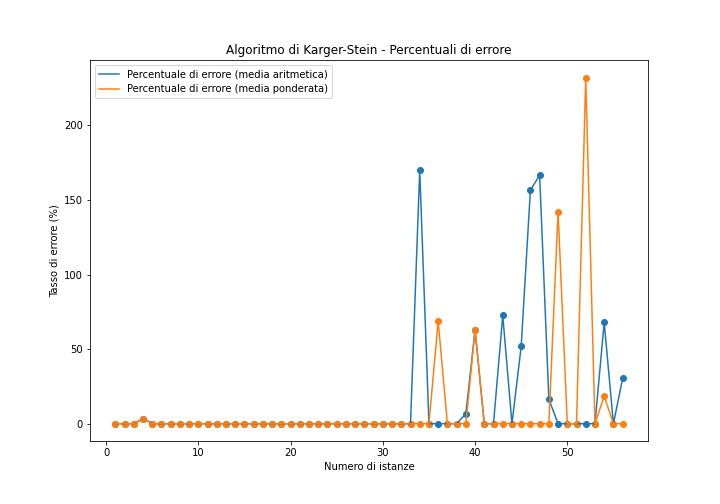
\includegraphics[width=1\textwidth]{res/images/single/karger-stein/tasso-di-errore/karger_stein_tassi_di_errore.png}
	\caption{Variazione del tasso di errore al variare della threshold
	(blu = threshold di 6 secondi, arancione = threshold di 10 secondi).}
	\label{fig:karger_stein_tassi_di_errore}
\end{figure}

\label{tabella_min_cut}
\begin{longtable}{llllllll}
	\textbf{Dataset} & \textbf{\begin{tabular}[c]{@{}l@{}}Correct\\ result\end{tabular}} & \textbf{\begin{tabular}[c]{@{}l@{}}Result w/o\\ threshold\end{tabular}} & \textbf{\begin{tabular}[c]{@{}l@{}}Error w/o\\ threshold\end{tabular}} & \textbf{\begin{tabular}[c]{@{}l@{}}Result\\ w/ 6s\end{tabular}} & \textbf{\begin{tabular}[c]{@{}l@{}}Error\\ w/ 6s\end{tabular}} & \textbf{\begin{tabular}[c]{@{}l@{}}Result\\ w/ 10s\end{tabular}} & \textbf{\begin{tabular}[c]{@{}l@{}}Error\\ w/ 10s\end{tabular}} \\
	\endhead
	%
	1 & 3056 & 3056 & 0.0 & 3056 & 0.0 & 3056 & 0.0 \\
	2 & 223 & 223 & 0.0 & 223 & 0.0 & 223 & 0.0 \\
	3 & 2302 & 2302 & 0.0 & 2302 & 0.0 & 2302 & 0.0 \\
	4 & 5152 & 5152 & 0.0 & 4974 & 3.45 & 4974 & 3.45 \\
	5 & 1526 & 1526 & 0.0 & 1526 & 0.0 & 1526 & 0.0 \\
	6 & 1684 & 1684 & 0.0 & 1684 & 0.0 & 1684 & 0.0 \\
	7 & 522 & 522 & 0.0 & 522 & 0.0 & 522 & 0.0 \\
	8 & 2866 & 2866 & 0.0 & 2866 & 0.0 & 2866 & 0.0 \\
	9 & 2137 & 2137 & 0.0 & 2137 & 0.0 & 2137 & 0.0 \\
	10 & 1446 & 1446 & 0.0 & 1446 & 0.0 & 1446 & 0.0 \\
	11 & 648 & 648 & 0.0 & 648 & 0.0 & 648 & 0.0 \\
	12 & 2486 & 2486 & 0.0 & 2486 & 0.0 & 2486 & 0.0 \\
	13 & 1282 & 1282 & 0.0 & 1282 & 0.0 & 1282 & 0.0 \\
	14 & 299 & 299 & 0.0 & 299 & 0.0 & 299 & 0.0 \\
	15 & 2113 & 2113 & 0.0 & 2113 & 0.0 & 2113 & 0.0 \\
	16 & 159 & 159 & 0.0 & 159 & 0.0 & 159 & 0.0 \\
	17 & 969 & 969 & 0.0 & 969 & 0.0 & 969 & 0.0 \\
	18 & 1756 & 1756 & 0.0 & 1756 & 0.0 & 1756 & 0.0 \\
	19 & 714 & 714 & 0.0 & 714 & 0.0 & 714 & 0.0 \\
	20 & 2610 & 2610 & 0.0 & 2610 & 0.0 & 2610 & 0.0 \\
	21 & 341 & 341 & 0.0 & 341 & 0.0 & 341 & 0.0 \\
	22 & 890 & 890 & 0.0 & 890 & 0.0 & 890 & 0.0 \\
	23 & 772 & 772 & 0.0 & 772 & 0.0 & 772 & 0.0 \\
	24 & 1561 & 1561 & 0.0 & 1561 & 0.0 & 1561 & 0.0 \\
	25 & 951 & 951 & 0.0 & 951 & 0.0 & 951 & 0.0 \\
	26 & 424 & 424 & 0.0 & 424 & 0.0 & 424 & 0.0 \\
	27 & 1153 & 1153 & 0.0 & 1153 & 0.0 & 1153 & 0.0 \\
	28 & 707 & 707 & 0.0 & 707 & 0.0 & 707 & 0.0 \\
	29 & 484 & 484 & 0.0 & 484 & 0.0 & 484 & 0.0 \\
	30 & 850 & 850 & 0.0 & 850 & 0.0 & 850 & 0.0 \\
	31 & 1382 & 1382 & 0.0 & 1382 & 0.0 & 1382 & 0.0 \\
	32 & 1102 & 1102 & 0.0 & 1102 & 0.0 & 1102 & 0.0 \\
	33 & 346 & 346 & 0.0 & 346 & 0.0 & 346 & 0.0 \\
	34 & 381 & 381 & 0.0 & 1028 & 169.82 & 381 & 0.0 \\
	35 & 129 & 129 & 0.0 & 129 & 0.0 & 129 & 0.0 \\
	36 & 670 & 670 & 0.0 & 670 & 0.0 & 209 & 68.81 \\
	37 & 1137 & 1137 & 0.0 & 1137 & 0.0 & 1137 & 0.0 \\
	38 & 869 & 869 & 0.0 & 869 & 0.0 & 869 & 0.0 \\
	39 & 868 & 868 & 0.0 & 926 & 6.68 & 868 & 0.0 \\
	40 & 1148 & 1148 & 0.0 & 1869 & 62.8 & 1869 & 62.8 \\
	41 & 676 & 676 & 0.0 & 676 & 0.0 & 676 & 0.0 \\
	42 & 290 & 290 & 0.0 & 290 & 0.0 & 290 & 0.0 \\
	43 & 818 & 818 & 0.0 & 1412 & 72.62 & 818 & 0.0 \\
	44 & 175 & 175 & 0.0 & 175 & 0.0 & 175 & 0.0 \\
	45 & 508 & 508 & 0.0 & 771 & 51.77 & 508 & 0.0 \\
	46 & 904 & 904 & 0.0 & 2320 & 156.64 & 904 & 0.0 \\
	47 & 362 & 362 & 0.0 & 965 & 166.57 & 362 & 0.0 \\
	48 & 509 & 509 & 0.0 & 593 & 16.5 & 509 & 0.0 \\
	49 & 400 & 400 & 0.0 & 400 & 0.0 & 968 & 142.0 \\
	50 & 364 & 364 & 0.0 & 364 & 0.0 & 364 & 0.0 \\
	51 & 336 & 336 & 0.0 & 336 & 0.0 & 336 & 0.0 \\
	52 & 639 & 639 & 0.0 & 639 & 0.0 & 2121 & 231.92 \\
	53 & 43 & 43 & 0.0 & 43 & 0.0 & 43 & 0.0 \\
	54 & 805 & 805 & 0.0 & 1352 & 67.95 & 954 & 18.51 \\
	55 & 363 & 363 & 0.0 & 363 & 0.0 & 363 & 0.0 \\
	56 & 584 & 584 & 0.0 & 761 & 30.31 & 584 & 0.0
	\end{longtable}

\subsection{Domanda 5}
\textit{Commentate i risultati che avete ottenuto: come si comportano gli algoritmi rispetto alle varie istanze? C'è un algoritmo che riesce sempre a fare meglio degli altri? Quale dei due algoritmi che avete implementato è più efficiente? Quale il più preciso nei risultati?}

I risultati ottenuti dai due algoritmi sono perfettamente in linea con quanto ci aspettavamo dal punto di vista della complessità teorica di ognuno. L'andamento delle varie istanze è in linea con la complessità teorica, visto che all'aumentare del numero di nodi aumenta in modo corrispondente il tempo di esecuzione dell'algoritmo da noi implementato. 
Analizzando i tempi di esecuzione dei due algoritmi possiamo affermare che l'algoritmo di Stoer e Wagner risulta essere nettamente più veloce rispetto a quello di Karger e Stein, con un tempo massimo nell'istanza più grande pari a poco più di un secondo (1.12 s per la precisione), mentre il secondo impiega più di 10 minuti (722.44 s) con le ripetizioni w.h.p. Quello di Stoer e Wagner è dunque l'algoritmo migliore su tutti i fronti (nello specifico, tempo computazionale e risultati ottenuti). Confrontandolo con Karger e Stein a livello di efficienza e precisione possiamo vedere che i risultati riportati sono corretti senza soglie di tempo impostate, mentre impostando delle soglie di 6 secondi e 10 secondi l'algoritmo ha un tasso di errore minore con soglie maggiori. Questo è triviale, essendo un algoritmo randomico w.h.p., e come ulteriore analisi possiamo vedere anche che quando si arriva a una grandezza pari a 250 nodi gli errori cominciano a manifestarsi, sebbene il tempo di esecuzione sia comunque superiore (anche in questo caso) rispetto a Stoer e Wagner. 
